\documentclass[tikz,border=8pt]{standalone}
\usepackage{amsmath,amssymb}
\usetikzlibrary{arrows.meta,automata,positioning,quotes}
\begin{document}
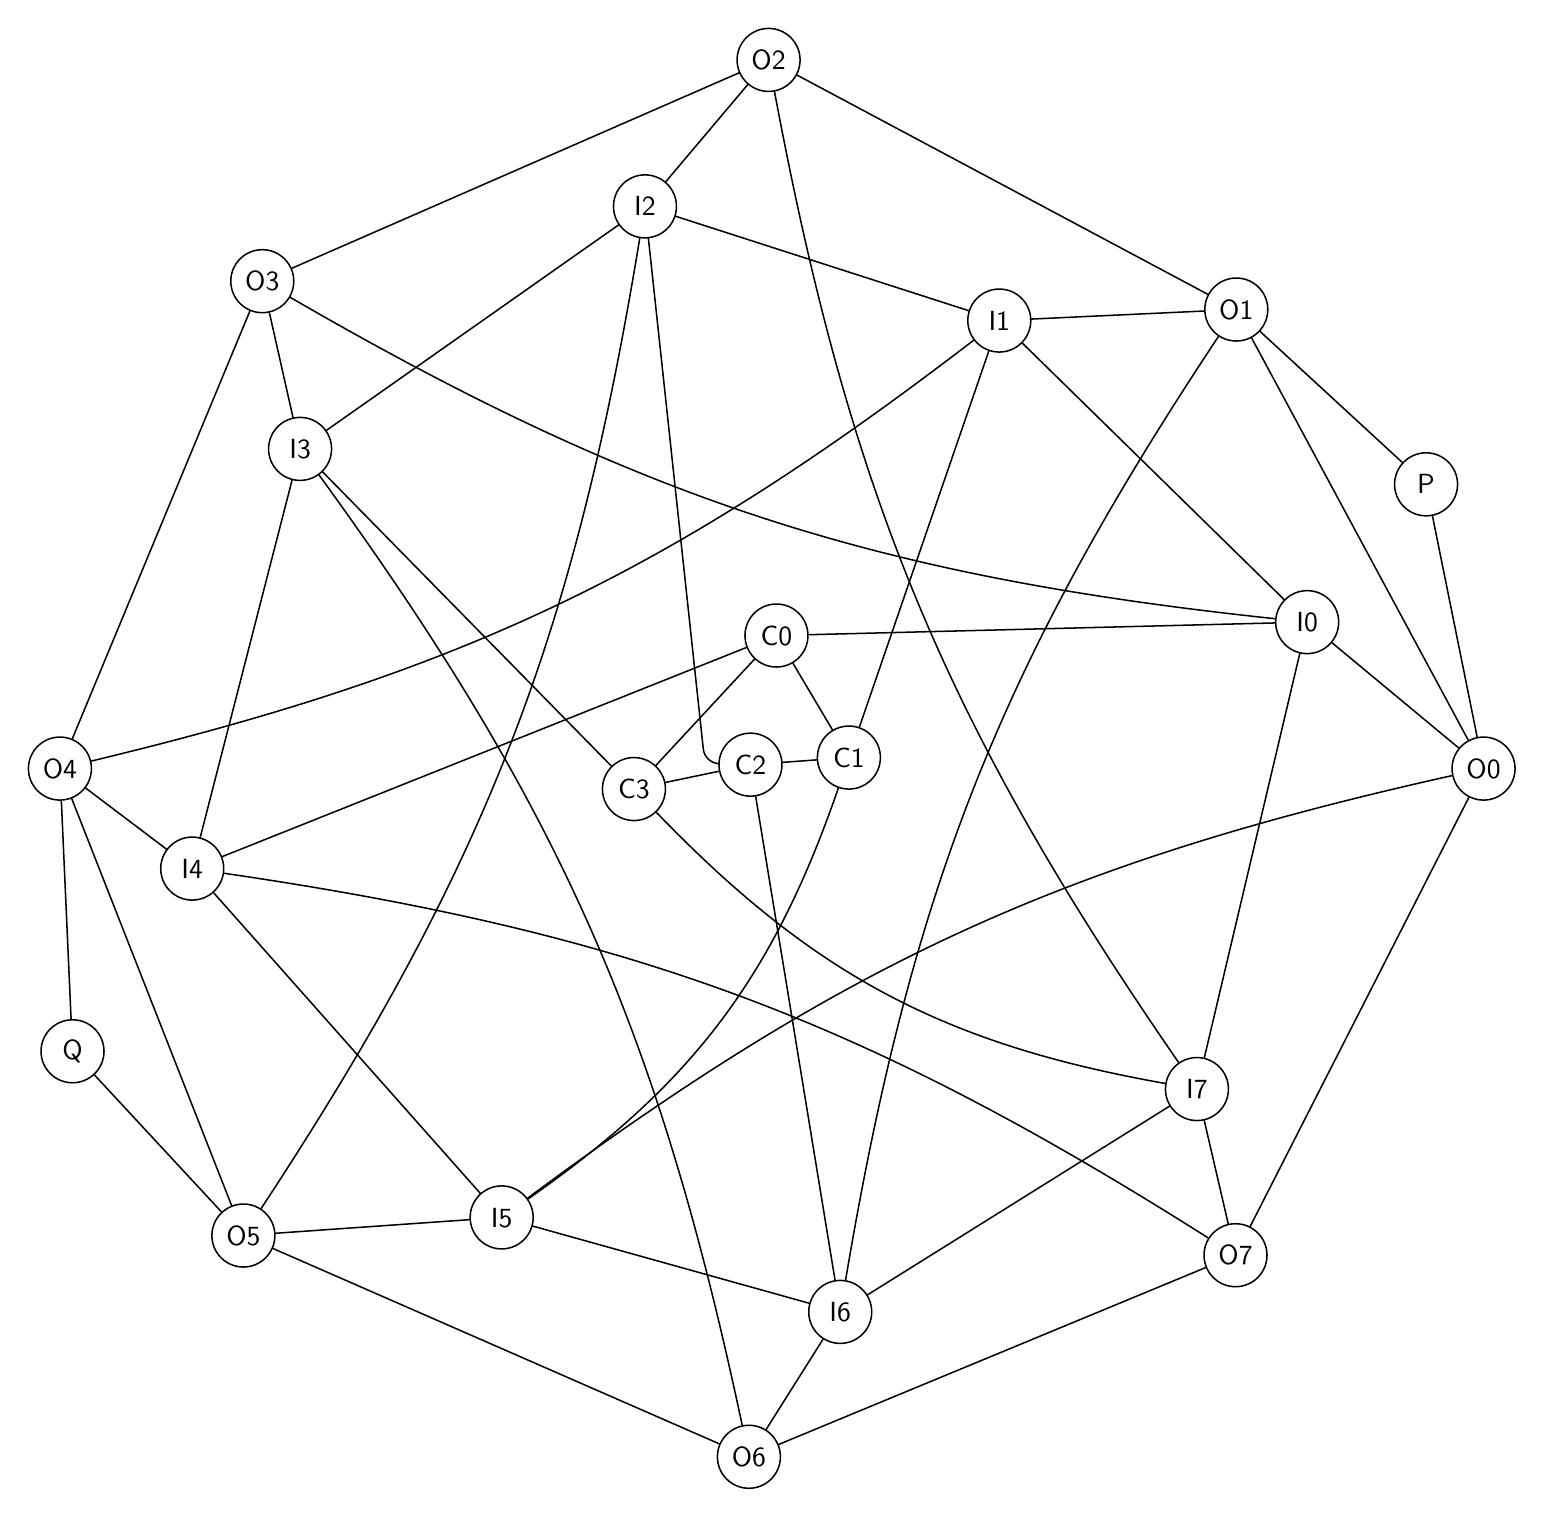
\begin{tikzpicture}[x=1cm,y=1cm]
\tikzset{
  graphnode/.style={circle,draw=black,line width=0.55pt,minimum size=8mm,inner sep=1pt,font=\sffamily},
  graphedge/.style={draw=black,line width=0.55pt,line cap=round,line join=round},
  directed/.style={graphedge,-{Stealth[length=2.4mm,width=2.0mm]}},
  undirected/.style={graphedge}
}
\node[graphnode] (n_O0) at (9.32,-0.03) {O0};
\node[graphnode] (n_O1) at (6.18,5.80) {O1};
\node[graphnode] (n_O2) at (0.24,8.97) {O2};
\node[graphnode] (n_O3) at (-6.19,6.16) {O3};
\node[graphnode] (n_O4) at (-8.76,-0.03) {O4};
\node[graphnode] (n_O5) at (-6.43,-5.96) {O5};
\node[graphnode] (n_O6) at (-0.01,-8.77) {O6};
\node[graphnode] (n_O7) at (6.17,-6.21) {O7};
\node[graphnode] (n_I0) at (7.08,1.83) {I0};
\node[graphnode] (n_I1) at (3.17,5.66) {I1};
\node[graphnode] (n_I2) at (-1.33,7.11) {I2};
\node[graphnode] (n_I3) at (-5.71,4.03) {I3};
\node[graphnode] (n_I4) at (-7.08,-1.30) {I4};
\node[graphnode] (n_I5) at (-3.15,-5.73) {I5};
\node[graphnode] (n_I6) at (1.15,-6.93) {I6};
\node[graphnode] (n_I7) at (5.68,-4.10) {I7};
\node[graphnode] (n_C0) at (0.34,1.66) {C0};
\node[graphnode] (n_C1) at (1.26,0.11) {C1};
\node[graphnode] (n_C2) at (0.01,0.02) {C2};
\node[graphnode] (n_C3) at (-1.47,-0.29) {C3};
\node[graphnode] (n_P) at (8.59,3.58) {P};
\node[graphnode] (n_Q) at (-8.60,-3.62) {Q};
\draw[undirected] (n_O0) -- (n_O1);
\draw[undirected] (n_O1) -- (n_O2);
\draw[undirected] (n_O2) -- (n_O3);
\draw[undirected] (n_O3) -- (n_O4);
\draw[undirected] (n_O4) -- (n_O5);
\draw[undirected] (n_O5) -- (n_O6);
\draw[undirected] (n_O6) -- (n_O7);
\draw[undirected] (n_O7) -- (n_O0);
\draw[undirected] (n_I0) -- (n_I1);
\draw[undirected] (n_I1) -- (n_I2);
\draw[undirected] (n_I2) -- (n_I3);
\draw[undirected] (n_I3) -- (n_I4);
\draw[undirected] (n_I4) -- (n_I5);
\draw[undirected] (n_I5) -- (n_I6);
\draw[undirected] (n_I6) -- (n_I7);
\draw[undirected] (n_I7) -- (n_I0);
\draw[undirected] (n_O0) -- (n_I0);
\draw[undirected] (n_O1) -- (n_I1);
\draw[undirected] (n_O2) -- (n_I2);
\draw[undirected] (n_O3) -- (n_I3);
\draw[undirected] (n_O4) -- (n_I4);
\draw[undirected] (n_O5) -- (n_I5);
\draw[undirected] (n_O6) -- (n_I6);
\draw[undirected] (n_O7) -- (n_I7);
\draw[undirected] (n_I0) to[bend left=12] (n_O3);
\draw[undirected] (n_I1) to[bend left=12] (n_O4);
\draw[undirected] (n_I2) to[bend left=12] (n_O5);
\draw[undirected] (n_I3) to[bend left=12] (n_O6);
\draw[undirected] (n_I4) to[bend left=12] (n_O7);
\draw[undirected] (n_I5) to[bend left=12] (n_O0);
\draw[undirected] (n_I6) to[bend left=12] (n_O1);
\draw[undirected] (n_I7) to[bend left=12] (n_O2);
\draw[undirected] (n_C0) -- (n_C1);
\draw[undirected] (n_C1) -- (n_C2);
\draw[undirected] (n_C2) -- (n_C3);
\draw[undirected] (n_C3) -- (n_C0);
\draw[undirected] (n_C0) -- (n_I0);
\draw[undirected] (n_C0) -- (n_I4);
\draw[undirected] (n_C1) -- (n_I1);
\draw[undirected] (n_C1) to[bend left=18] (n_I5);
\draw[undirected,rounded corners=5pt] (n_C2) -- (-0.57,0.04) -- (n_I2);
\draw[undirected] (n_C2) -- (n_I6);
\draw[undirected] (n_C3) -- (n_I3);
\draw[undirected] (n_C3) to[bend right=18] (n_I7);
\draw[undirected] (n_P) -- (n_O0);
\draw[undirected] (n_P) -- (n_O1);
\draw[undirected] (n_Q) -- (n_O4);
\draw[undirected] (n_Q) -- (n_O5);
\end{tikzpicture}
\end{document}
